% !TEX encoding = UTF-8 Unicode
% !TeX spellcheck = it
\documentclass[a4paper,8pt]{article}
\usepackage[italian]{babel}
\usepackage{graphicx}
\usepackage{blindtext}
\usepackage[T1]{fontenc}
\usepackage[utf8x]{inputenc}
\usepackage{multicol, caption}
\usepackage[none]{hyphenat}
\usepackage{hyperref}
\usepackage[margin={3cm,1cm}]{geometry}
\usepackage{titlesec}
\usepackage{tabularx} % for 'tabularx' environment
\graphicspath{ {images/} }
\newenvironment{Figure}
  {\par\medskip\noindent\minipage{\linewidth}}
  {\endminipage\par\medskip}

\newenvironment{Table}
   {\par\bigskip\noindent\minipage{\linewidth}\centering}
   {\endminipage\par\bigskip}

\setlength{\columnsep}{1cm}

\hypersetup{
	colorlinks=true,
	allcolors=[rgb]{0.376,0.49,0.54}
	%urlcolor=[rgb]{0,0,0}
}

\titleformat{\section}
{\normalfont\fontsize{11}{11}\bfseries}
{\thesection.}{1em}{}

\titleformat{\subsection}
{\normalfont\fontsize{9}{9}\bfseries}
{\thesubsection.}{1em}{}

\begin{document}
\title{Comparazione di classificatori in Credit Card Approval}
\author{Valerio Colitta, Daniele Cominu, Alessio Fiorenza}
\date{Aprile 2017}
\maketitle

%TODO: inserire un indice con i vari link alle section.%

\begin{multicols}{2}

\section{Descrizione preliminare}
Volendo approfondire i metodi e le tecniche di classificazione affrontate nel corso di Metodi Quantitativi per l'Informatica, abbiamo deciso di confrontarli risolvendo il problema presentato in \emph{Credit Approval Data Set} \cite{Dataset}; abbiamo deciso di utilizzare modelli di diverse complessità ed abbiamo osservato che data la conformazione dei dati e la loro dimensione ridotta, si ottengono risultati migliori con modelli meno complessi. 

\section{Il dataset}
Il dataset riguarda delle domande di approvazione di carte di credito, ed e' composto da 690 campioni, 37 dei quali con valori mancanti. Sono presenti in totale 15 feature, le quali si articolano in 6 continue e 9 categoriche. Tali dati sono poi classificati in due classi \{+, -\} che rappresentano rispettivamente l'approvazione o meno della carta di credito.
Il significato delle 15 feature non è noto per poter mantenere la confidenzialità dei dati.

\section{Manipolazione dei dati}
Come prima cosa sono stati eliminati manualmente dal dataset i 37 campioni di cui non erano stati specificate alcune feature, riducendo ulteriormente la dimensione del dataset a 653 campioni.\\
\subsection{One Hot Encoding}
Per superare l'eterogeneità nella tipologia delle feature, si è deciso di applicare la tecnica del \emph{One Hot Encoding} \cite{OneHotEncoding} per le feature categoriche; l'\emph{One Hot Encoding} è una tecnica utilizzata per trattare feature categoriche in problemi di classificazione e regressione, e consiste nel tradurre una feature categorica che può assumere \emph{n} valori distinti in un vettore di \emph{n} feature binarie; per ogni campione la feature i-esima del vettore calcolato assume il valore 1 se e solo se il campione assume il valore i-esimo per la feature considerata; le restanti \emph{n }- 1 sono dunque settate a 0 per tale campione.
Se si fosse utilizzata una feature a valori reali, in cui per ogni valore assunto dalla feature viene associato un numero reale, sarebbero state introdotte delle distanze diverse tra i valori assunti dalla feature; Ad esempio, considerando una feature categorica che descrive la specie di appartenenza, mappando i valori assunti a dei numeri incrementali, si può notare come si introduca una maggiore distanza tra i campioni (2, 7) rispetto ai campioni (4, 5).
\begin{Figure}
 \centering
 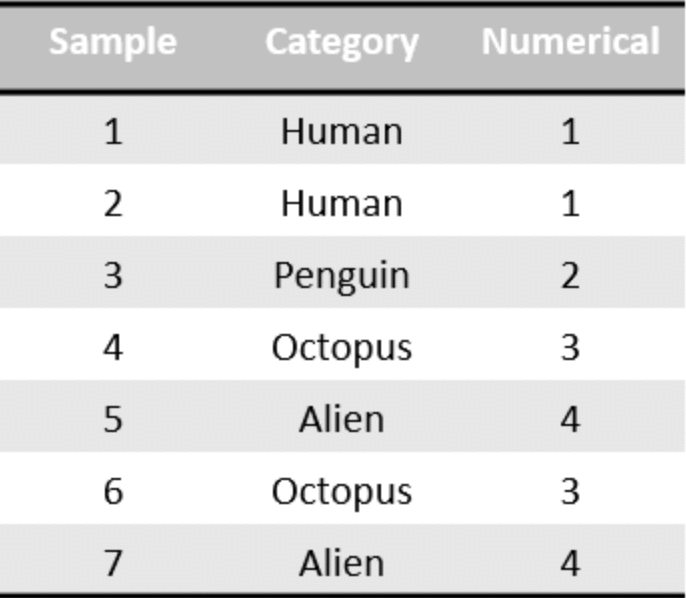
\includegraphics[width=\linewidth]{categbw}
 \captionof{figure}{mapping categorica -> reale}
\end{Figure}
Introducendo il one hot encoding si può notare come le distanze tra i campioni (2,7) e (4,5) siano le stesse\\
\begin{Figure}
 \centering
 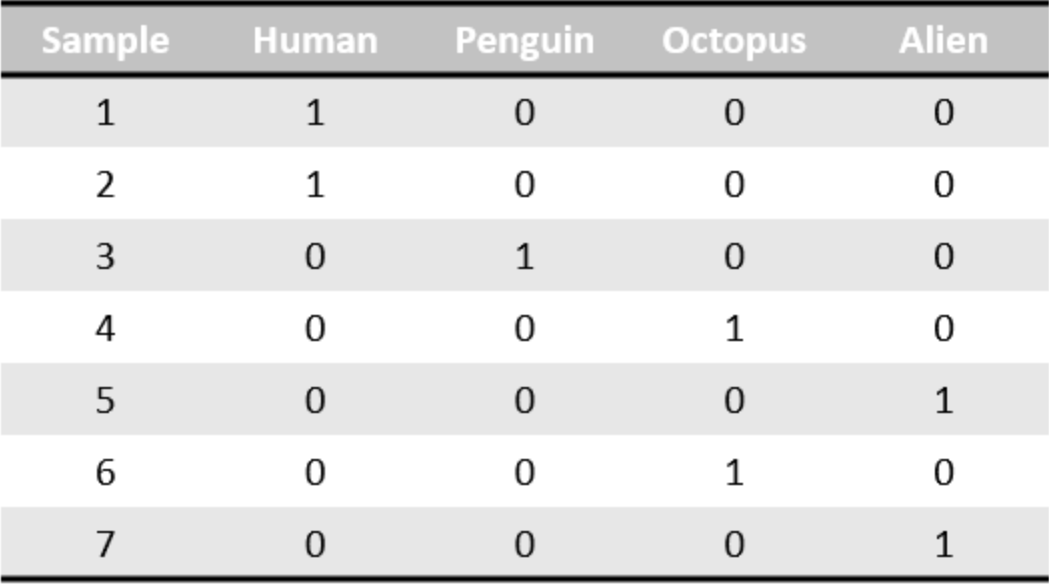
\includegraphics[width=\linewidth]{categvecbw}
 \captionof{figure}{one hot encoding}
\end{Figure}

\subsection{Standardizzazione}
Successivamente all'one hot encoding, è seguita la fase di standardizzazione delle variabili; per ogni feature sono stati calcolati la media campionaria $\mu$ e la deviazione standard campionaria $\sigma$, definite come: 
\begin{equation}
	\mu_{j} = \frac{1}{N}\sum_{i=1}^{N} x_{ij}
\end{equation}
 
\begin{equation}
	\sigma_{j} = \sqrt{\frac{1}{N-1}\sum_{i=1}^{N}(x_{ij} - \mu_{j})^2}
\end{equation} 

Una volta calcolati questi due valori, i campioni vengono standardizzati attraverso la seguente formula:
\begin{equation}
	x_{ij} = \frac{x_{ij} - \mu_{j}}{\sigma_{j}}
\end{equation}

Questa trasformazione fa si che le nuove feature abbiano valor medio $\mu$ nullo e varianza $\sigma^2$ unitaria;  ciò è necessario poiché alcuni metodi utilizzano la distanza euclidea e potrebbero essere ingannati dall'utilizzo di diverse scale per le diverse feature. %Le feature con varianza elevata avranno più importanza di altre% 

\section{Principal Component Analysis}

\section{Visualizzazione dei dati}
In genere risulta estremamente utile effettuare una visualizzazione dei dati prima di procedere all'applicazione dei modelli, in modo da individuare pattern utili per guidare il processo di selezione del modello e l'analisi dei risultati ottenuti. I grafici in Figura 3 rappresentano le distribuzioni dei campioni considerando coppie di feature continue; ossia nella cella presente alla riga \emph{i-esima} e colonna \emph{j-esima} è presente un grafico in cui sull'asse x sono riportati i valori assunti dalla feature \emph{j-esima}, sull'asse y quelli assunti dalla feature \emph{i-esima} .

\begin{Figure}
 \centering
 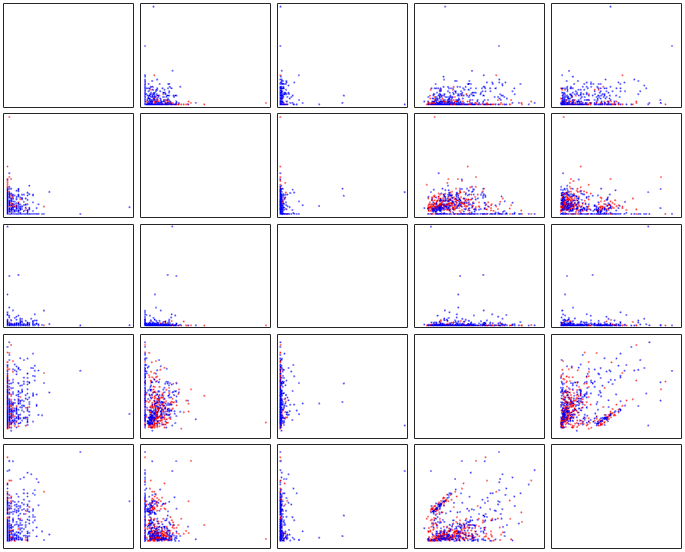
\includegraphics[width=\linewidth]{mcov}
 \captionof{figure}{}
\end{Figure}

Dai grafici non si evincono particolari legami tra le feature. E' pertanto necessario continuare ad investigare. %temporaneo...%
\section{Modelli utilizzati}
Si è deciso di affrontare il problema utilizzando diversi modelli, in modo da poter approfondire la struttura del problema proposto. Si è notato come modelli più semplici riescano a generalizzare maggiormente a fronte di nuovi dati di input, e ciò è dovuto a diversi fattori, tra cui la dimensione ridotta del dataset e il numero relativamente alto di feature.
Prima del training il dataset è stato inizialmente diviso in due parti: \emph{Training set} (80\%) e \emph{Test set} (20\%), utilizzati rispettivamente per il training e la selezione degli iperparametri attraverso la cross-validation e il test dei risultati ottenuti.\\
Nella Tabella 1 sono riportati gli error-rate medi e minimi ottenuti applicando i diversi modelli.\\
\begin{Table}
\small
   \begin{tabular}{|p{4.1cm}|p{0.8cm}|p{0.8cm}|}
\hline
 \multicolumn{1}{|c|}{\textbf{\scalebox{0.9}{Modello}}} & \multicolumn{1}{c}{\textbf{\scalebox{0.9}{Min}}} & \multicolumn{1}{|c|}{\textbf{\scalebox{0.9}{Med}}}\\ \hline
    	\scalebox{0.9}{Linear Discriminant Analysis}& 10.12 & 10 \\ \hline
	\scalebox{0.9}{Quadratic Discriminant Analysis} & 10 & 10\\ \hline
	\scalebox{0.9}{Diagonal Discriminant Analysis} & 0.04 & 0.224\\ \hline
\scalebox{0.9}{Logistic Regression (LB)} & 10 & 10 \\ \hline
	\scalebox{0.9}{Logistic Regression (QB)} & 10 & 10 \\ \hline
	\scalebox{0.9}{Logistic Regression (LBR)} & 10 & 10 \\ \hline
	\scalebox{0.9}{Logistic Regression (QBR)} & 10 & 10 \\ \hline
   \end{tabular}
  \captionof{table}{errori minimi e medi dei modelli utilizzati}
\end{Table}
\section{Gaussian Discriminant Analysis}
La Gaussian Discriminant Analysis, o GDA, è una tecnica di classificazione di tipo \emph{generativa}, nel senso che cerca di calcolare (attraverso Maximum Likelihood Estimation) la distribuzione $p(x | y)$ di una serie di campioni, a partire dalla loro classe $y$ di appartenenza. Con la GDA, si assume che i campioni di ogni classe \emph{c} siano distribuiti come delle Gaussiane Multivariate, nel senso che
\begin{equation}
p(x|y=c) \sim \mathcal{N}(\mu_{c},\,\Sigma_{c})\quad \forall{c} \in \{1, ..., C\}
\end{equation}
dove $\mu_{c}$ rappresenta il vettore dei valori medi della distribuzione, e $\Sigma_{c}$ la matrice di covarianza delle feature.
%SCRIVI IL TEOREMA DI FREDA%
%DIFFERENZE TRA GENERATIVO E DISCRIMINATIVO%
Una volta trovati i due parametri $(\mu, \Sigma)$, per classificare un nuovo input $x_{0}$ in una delle $C$ classi viene calcolato
\begin{equation}
\arg\max_{c}p(y = c|x = x_{0}) \quad \forall{c} \in \{1, ..., C\}
\end{equation}
e cioè la massima probabilità che la classe di appartenenza di $x_{0}$ sia \emph{c}, per tutte le $C$ classi.
\subsection{Linear Discriminant Analysis}
\subsection{Quadratic Discriminant Analysis}
\section{Logistic Regression}
\subsection{Linear Boundary}
\subsection{Quadratic Boundary}
\subsection{Regolarizzazione}
\section{Bias vs Variance}
\end{multicols}

\begin{thebibliography}{10}
\bibitem{Dataset}
	John Ross Quinlan \\
	\emph{Credit Approval Data Set} \\
	\url{http://archive.ics.uci.edu/ml/datasets/Credit+Approval}
\bibitem{OneHotEncoding}
	Håkon Hapnes Strand \\
	\emph{One Hot Encoding} \\
	\url{https://www.quora.com/What-is-one-hot-encoding-and-when-is-it-used-in-data-science}
	
\end{thebibliography}
\end{document}